\chapter{Recurrent Neural Networks}

Recurrent Neural Networks (RNN) can be used in a wide variety of tasks as they can work with inputs and outputs of variable size.
\begin{figure}[H]
    \centering
    \includegraphics[width=\textwidth]{Images/rnn.jpeg}
    \caption{The applications of Recurrent Neural Networks \cite{unres-rnn}}
\end{figure}

\begin{enumerate}
     \itemsep0em
     \item \textbf{One to one}: A vanilla neural network with fixed-sized input and fixed-sized output.
     \item \textbf{One to many}: An RNN with sequence output, e.g. image captioning: generate a sentence describing an input image.
     \item \textbf{Many to one}: An RNN with sequence input, e.g. sentiment analysis: infer the emotion of a given sentence.
     \item \textbf{Many to many (1)}: Sequence input and sequence output, e.g.: machine translation: output a sentence in Spanish given a sentence in English.
     \item \textbf{Many to many (2)}: Synced sequence input and output, e.g.: video classification: label each frame of a video.
\end{enumerate}

%%%%%%%%%%%%%%%%%%%%%%%%%%%%%%%%%%%%%%%%%%%%%%%%%%%%%%%%%%%%
%%%%%%%%%%%%%%%%%%%%  NEW SECTION   %%%%%%%%%%%%%%%%%%%%%%%%
%%%%%%%%%%%%%%%%%%%%%%%%%%%%%%%%%%%%%%%%%%%%%%%%%%%%%%%%%%%%
\section{Vanilla RNN}
Traditional neural networks do not have any memory as each input of the network are independent. Recurrent neural networks use loops to make information persist as shown on Figure (\ref{vanilla-rnn}).

\begin{figure}[H]
    \centering
    \includegraphics[width=0.3\textwidth]{Images/vanilla-rnn.png}
    \caption{A vanilla recurrent neural network \cite{colah}}
    \label{vanilla-rnn}
\end{figure}

Given an input $x_t$ and a layer $A$, the output $h_t$ is fed again to the layer along with the next input $x_{t+1}$. This becomes clearer when we unroll the RNN:

\begin{figure}[H]
    \centering
    \includegraphics[width=\textwidth]{Images/vanilla-rnn2.png}
    \caption{An unrolled vanilla recurrent neural network \cite{colah}}
\end{figure}

Basically, if we denote the function of the layer A by $f$:
\begin{equation}
    h_t = f(h_{t-1}, x_t)
\end{equation}

Suppose the input $x_t \in \mathbb{R}^{D}$ and the layer $A$ contains $H$ neurons. Denote $W_x \in \mathbb{R}^{D\times H}$ the weights of the input, and $W_h \in \mathbb{R}^{H\times H}$ the weights of the hidden state. Usually $f$ is simply:
\begin{equation}
    h_t = \text{tanh}(W_x x_t + W_h h_{t-1})
\end{equation}

Just like the layer traditional neural network with a tanh (hyperbolic tangent) activation function and two inputs instead of one.

\begin{figure}[H]
    \centering
    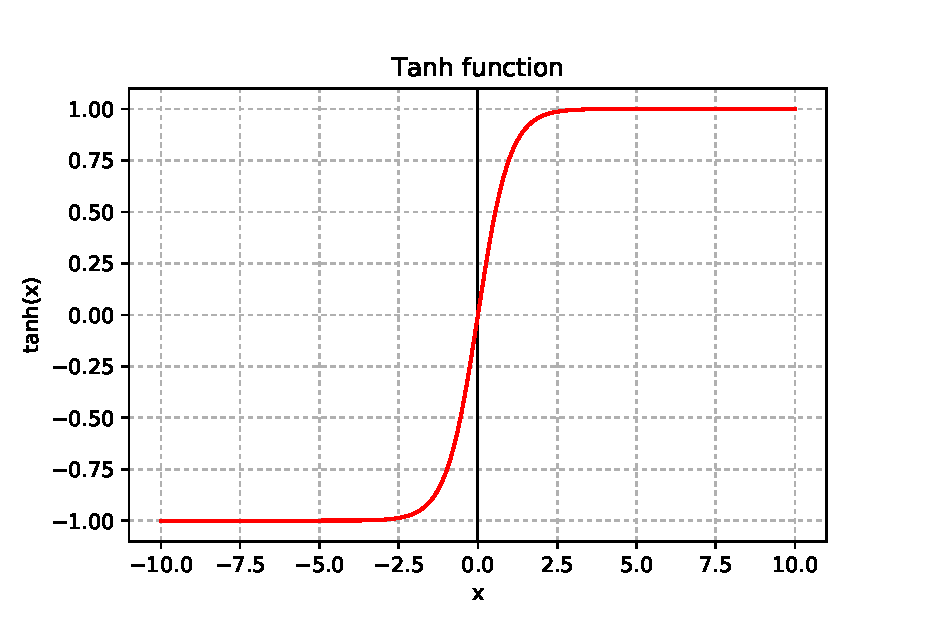
\includegraphics[width=0.5\textwidth]{Images/tanh.eps}
    \caption{Another activation function: tanh}
\end{figure}

This vanilla RNN is a good step towards learning from sequential inputs but most people use a variant called Long-Short Term Memory (LSTM) that work extremely well on many different tasks. 

\section{Long-Short Term Memory Networks}
The vanilla RNN is hard to train as the gradients often either vanish or explode. That's because during backpropagation, the weights $W_x$ and $W_h$ go through repeated matrix multiplication [detail the maths] than can either make them go to zero or diverge. LSTMs solve this problem by using a gating mechanism. 

They keep track of the hidden state vector $h_t \in \mathbb{R}^H$ but also of a cell state vector $c_t\in \mathbb{R}^H$, we'll shortly explain. First, we compute the activation vector $a \in \mathbb{R}^{4H}$ that is 4 times bigger than vanilla RNN, which is necessary to remember long and short-term features. 
\begin{equation}
a = W_x x + W_h h
\end{equation}
with $x \in \mathbb{R}^{D}$, the input, $h \in \mathbb{R}^{H}$, the hidden state, $W_x \in \mathbb{R}^{D\times 4H}$ and $W_h \in \mathbb{R}^{H\times 4H}$.

Then this activation vector $a$ is split into 4: $a_i, a_f, a_o, a_g \in \mathbb{R}^H$, where $a_i$ is made up of the first $H$ elements of $a$, $a_f$ the $H$ next, etc. Now we compute the input gate $i \in \mathbb{R}^H$, the forget gate $f \in \mathbb{R}^H$, the output gate $o \in \mathbb{R}^H$ and the block input $g \in \mathbb{R}^H$ as: 
\begin{equation}
    i = \sigma(a_i) \qquad f = \sigma(a_f) \qquad o = \sigma(a_o) \qquad g = \text{tanh}(a_g)
\end{equation}
where $\sigma$ is the sigmoid function.

Finally, we can compute the new cell state and the new hidden state as follow:
\begin{equation}
     c_t = i\odot g + f\odot c_{t-1} \qquad h_t = o\odot \text{tanh}(c_t)
\end{equation}
where $\odot$ is the elementwise product of vectors.
$c_t$ is the sum of:
\begin{itemize}
    \item The new information $g$ weighted by how much we want to add that new information with $i$ (remember that the sigmoid function has values between 0 and 
    1).
    \item What we knew before, $c_{t-1}$, weighted by how much we want to forget long-term information with $f$.
\end{itemize} 
That cell state then goes through a tanh activation function (just like in the vanilla RNN) and is multiplied by the output gate $o$ that decide how much to let through the next state. 

LSTMs therefore manage to easily remember long-term dependencies, as well as short-term ones, thus its name.

Also, note that the activation function in recurrent neural networks is a tanh and not a ReLU. ReLU was originally introduced to replace tanh because of the vanishing gradient problem. However, in the case of recurrent networks, LSTMs are built to not have vanishing gradients, which makes ReLU unnecessary.

\newpage
\section{LSTM for Sentiment Analysis}
We'll be using the following architecture:

\begin{figure}[H]
    \centering
    \includegraphics[width=0.3\textwidth]{Images/many-to-one.png}
    \caption{Many to one architecture}
\end{figure}

Each post will be broken down into a sequence of words and then fed to the LSTM that will infer the emotion of the user. On a more technical note, the vector of words will be represented by a list of ids from the Word2Vec vocabulary say $[3, 20, 1, 49, 6]$. To account for shorter posts, we'll have to zero-pad the vector -- the id 0 will actually be associated with a word token $<$PAD$>$ -- as $[3, 20, 1, 49, 6, 0, 0, ..., 0]$. The LSTM will then give the prediction by stopping before the zero-padding.

\section{Results}
(upcoming)







